%En esta ocasión es de interés resaltar la forma como se gestiona el
%proyecto, tema que uds. ya avanzaron en la preparación y ejecución del
%"workshop".

\subsection{Metodologías de trabajo}

Es necesario comprender que la mayoría de los proyectos realizados,
tienen una estructuración similar, lo que beneficia positivamente a la hora
de ejercer un control o división de tareas.

Por lo general cada equipo de trabajo está formado de una persona
a cargo del proyecto y en promedio 3 otras personas que cumplirían
la labor de ser un desarrollador activo del proyecto.

Con respecto a la metodología de trabajo que se utiliza
en todo el grupo, poder afirmar que se siguen una secuencia determinada,
al momento de efectuar el desarrollo.

\begin{itemize}
    \item Actividades a realizar:

			Se definen un conjunto de actividades dentro de los horarios
			dispuestos por todos los integrantes de cada proyecto, estos
			pueden ser tanto presenciales como remotos. Dichas actividades
			presentan gran flexibilidad a la hora definir en que momento
			realizarlas.
    \item Cada actividad hace uso de una herramienta:

			Desde el tomar acta de una reunión, hasta la programación
			se hace considerando el uso de una determinada herramienta,
			como las que veremos más adelante, he aquí el corazón de la
			investigación, pues las herramientas son la columna vertebral
			de la gestión y organización de un proyecto, para lograr que 
			todo funcione con la menor incertidumbre posible.
    \item Por cada herramienta, existe una previa capacitación:

			En primera instancia, cuando una persona se integra,
			tiene la facilidad de poder comenzar a utilizar las herramientas
			a modo de prueba, siendo instruido por otro miembro del grupo
			para no dejar dudas y completar la familiarización. Se suele
			dejar en un lugar centralizado (sitio web), pequeños tutoriales
			que ayudan a la persona nueva, a interiorizarse de manera más
			rápida con las herramientas.
    \item Las actividades son claras y cortas.

			Si bien es cierto el desarrollo de un proyecto es un largo camino,
			al momento de tener ciertos horarios en la semana para trabajar
			es recomendable poder definir objetivos a corto plazo, y así
			poder cumplirlos en poco tiempo. Esto ayuda en sobremanera
			a la autorrealización de cada integrante, pues puede recibir
			reconocimiento por realizar poco trabajo pero de calidad.
			Además el poder realizar un trabajo ``Lento pero seguro'',
			garantiza la construcción de unos buenos cimientos para el
			proyecto en desarrollo.
\end{itemize}


\subsection{Herramientas}

\begin{itemize}
	\item \textbf{TRAC}~\footnote{\url{http://trac.edgewall.org}}
	
	\begin{center}
    	
\includegraphics[width=0.15\textwidth]{../3-workshop/1-metodologia/img/trac}
	\end{center}

	Es una herramienta web para la gestión de proyectos,
	que tiene la característica de ser Open Source.

	La gracia de esta herramienta es la correcta integración,
	con sistema de control de versiones, Wikis, sistemas
	de tickets (bugtracker), Timelines, Roadmaps, etc.

	\item \textbf{Planner}~\footnote{\url{http://live.gnome.org/Planner}}

	\begin{center}
	    
\includegraphics[width=0.1\textwidth]{../3-workshop/1-metodologia/img/planner}
	\end{center}

	Es una herramienta para planear, programar y seguir el desarrollo de proyectos,
	teniendo la característica principal de ser Open Source.

	Como funciones principales, Planner nos permite la gestión de calendarios,
	gestión de recursos, seguimiento  de los avances del proyecto, enlace de tareas,
	exportación de documento como la carta gantt, a distintos formatos.
	
	\item \textbf{Git}~\footnote{\url{http://git-scm.com/}}

	\begin{center}
	    
\includegraphics[width=0.2\textwidth]{../3-workshop/1-metodologia/img/git}
	\end{center}


	Software enfocado al control de versiones de distintos proyectos,
	se caracteriza por ser el mecanismo principal del desarrollo del kernel
	del sistema operativo Linux. Además nos permite tener una gestión 
	distribuida, apoyando el desarrollo no-lineal y el poder trabajar
	de manera offline.

	Posee la característica de permitir la publicación en varios formatos,
	y una gran compatibilidad e integración con otros softwares de desarrollo.

	\item \textbf{LaTeX}~\footnote{\url{http://www.latex-project.org/}}

	\begin{center}
	    
\includegraphics[width=0.2\textwidth]{../3-workshop/1-metodologia/img/latex}
	\end{center}

	Esta herramienta es un sistema de composición de textos científicos,
	siguiendo estándares para poder ser válido inclusive como publicaciones
	o libros científicos, es actualmente usado en conferencias de organizaciones
	como la IEEE.

	Es un proyecto Open Source y permite la composición de textos distribuidos,
	es por esto la gran afinidad a las demás herramientas nombradas en esta sección.

	Al ser un formato en el cual se escribe en texto plano, es muy útil si se utiliza
	con un software de control de versiones, debido a que permite el trabajo
    colaborativo de manera mas sencilla, con la resultante ventaja de manejar versiones.

	\item \textbf{Skype}~\footnote{\url{http://www.skype.com/}}

	\begin{center}
	    
\includegraphics[width=0.2\textwidth]{../3-workshop/1-metodologia/img/skype}
	\end{center}


	Skype es un software para realizar llamadas VoIP, y la característica principal
	es que se pueden realizar llamadas, tanto entre usuarios Skype como a teléfonos
	móviles o fijos de todo el mundo.

	Es especial para poder realizar video y tele conferencias,
	es ahí la afinidad con la realización y desarrollo de proyectos internacionales
	de forma distribuida.

\end{itemize}

Los tutoriales se encuentran en el apartado~\ref{sec:anexos2}.

\subsection{Monitoreo y Seguimiento de proyectos}

El monitorio y los distintos mecanismo de seguimiento de los proyectos,
es un factor fundamental pues es el único mecanismo directo para poder
ver la evolución de una determinada tarea y a la misma vez, nos sirve
para ver el desempeño de cada integrante del equipo.

Cada semana, se realiza como mínimo una reunión por cada proyecto,
en las cuales se verifican los avances, se aclaran dudas, se discuten
problemáticas que puedan ir surgiendo con el tiempo y también
se recurre a una re-planificación en caso de ser necesaria.

Por otro lado, cada miembro tiene como obligación la creación
de un \emph{Worklog} de trabajo, cada vez que realiza cualquier
tipo de actividad, desde la lectura de una determinada publicación
hasta el poder programar alguna funcionalidad necesaria para un software.

De esta forma, este medio de comunicación pasivo, sirve para poder
dejar registro del trabajo realizado, a la vez sirve de documentación
del proyecto y de la misma forma, vamos dejando documentación que 
para cualquier miembro del equipo puede ser útil, por ejemplo, la corrección
de un error frecuente, por lo tanto, si nos damos cuenta estamos
realizando una suerte de traspaso de conocimiento, de una forma
indirecta, y a la vez verificando el trabajo.

Recordemos que desde tiempos inmemoriales, las bitácoras han sido útiles,
ya sea como elemento fundamental de la historia, o como vestigio
de algún hecho o avance en la historia de la humanidad.

\subsection{Espacio de Trabajo}

El hecho de gestionar un proyecto, no deja de lado la importancia
que implica el contar con un espacio de trabajo acorde a lo que desea realizar.

En este caso, se cuenta con un laboratorio que esta completamente equipado con
estaciones de trabajo (PC), conectividad a la red, etc.

Toda esta infraestructura se debe estar constantemente controlando,
dependiendo de las necesidades que posea
cada equipo de trabajo, desde la comodidad a la hora de trabajar, como de necesitar
un software en particular, hasta las características de un equipo en particular.

Esto da a entender que no sólo es necesario identificar
la manera adecuada de trabajar para cada equipo, sino que se hace imperativo
entregarles todo lo necesario para su normal funcionamiento.

Con responsabilidad adicional de cada miembro, está el poder mantener el espacio
de trabajo de una forma ordenada y limpio, pues al ser un espacio común, la falta
de cualquier persona afecta negativamente a todo el equipo de trabajo.

\subsection{Encuesta}

La siguiente encuesta está relacionada con el uso
de las herramientas anteriormente descritas, a modo
de poder obtener retroalimentación en el procedimiento
de gestión de proyectos, y de  la misma forma, poder
mejorar el desempeño y organización del equipo de trabajo.

\subsubsection{Inicio (para la generación de ideas)}
\begin{enumerate}
	\item ¿Cuál cree usted que es la mejor técnica o
		metodología de trabajo para la generación de
		ideas?
		\begin{enumerate}
			\item Brainstorming
			\item Encuestas
			\item Método Delphi
			\item Reunión de trabajo presencial
			\item Videoconferencia
			\item Other: 
		\end{enumerate}
        \begin{center}
        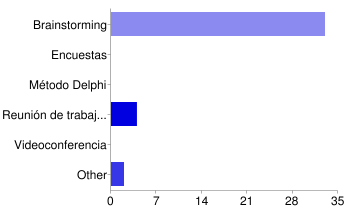
\includegraphics[scale=0.7]{images/encuesta2/1}
        \end{center}
	\item ¿Cuál cree usted que es la mejor forma de
		llevar a cabo la toma de decisiones en un
		equipo?
		\begin{enumerate}
			\item El jefe decide
			\item Votaciones
			\item Discusión abierta, con argumentos
				para cada propuesta
			\item Other: 
		\end{enumerate}
        \begin{center}
        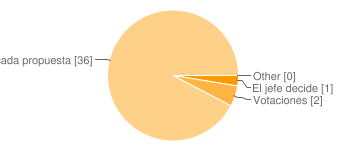
\includegraphics[scale=0.7]{images/encuesta2/2}
        \end{center}
	\item ¿Cuál cree usted que es el mejor mecanismo
		de capacitación para los nuevos integrantes?
		\begin{enumerate}
			\item Entrega de documentos
			\item Workshop de introducción
			\item Sin mecanismo (la persona nueva se acerca a preguntar)
			\item Other: 
		\end{enumerate}
        \begin{center}
        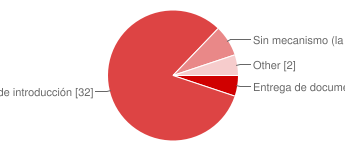
\includegraphics[scale=0.7]{images/encuesta2/3}
        \end{center}
\end{enumerate}

\subsubsection{Plan}

\begin{enumerate}
	\item ¿Considera eficiente el uso de planner
		y TRAC a la hora de realizar la planificación
		de un proyecto?
		\begin{verbatim}
            1		 2		 3		 4		 5
        Ineficiente						Muy Eficiente
		\end{verbatim}
        \begin{center}
        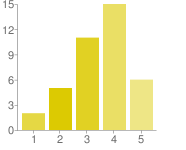
\includegraphics[scale=0.7]{images/encuesta2/4}
        \end{center}
	\item ¿Considera que se puede llevar a cabo un
		proyecto exitosamente sin realizar una
		planificación detallada?

		\begin{verbatim}
        1					 2					 3				 4					 5
        No, se requiere una meticulosa planificación						Si, no es necesario.
		\end{verbatim}
        \begin{center}
        
\includegraphics[scale=0.7]{images/encuesta2/5}
        \end{center}

	\item ¿Es planner una herramienta robusta para
		la creación de cartas gantt?
	
		\begin{verbatim}
               1		2		3		4		5
         No, muy mala				Si, Excelente
		\end{verbatim}
        \begin{center}
        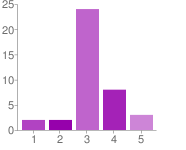
\includegraphics[scale=0.7]{images/encuesta2/6}
        \end{center}
\end{enumerate}

\subsubsection{Ejecución}

\begin{enumerate}
	\item ¿Cuál considera usted que es la base
		para la ejecución exitosa de un proyecto?
		\begin{enumerate}
			\item Reuniones frecuentes
			\item Uso de herramientas correctas
			\item División de trabajo
			\item Discusión de ideas
			\item Other: 
		\end{enumerate}
        \begin{center}
        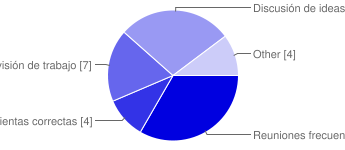
\includegraphics[scale=0.7]{images/encuesta2/7}
        \end{center}
	\item ¿Considera que un software de control de
		versiones es útil para desarrollar un
		proyecto informático?
		\begin{verbatim}
           1	2	3	4	5
        Inútil			Muy Útil
		\end{verbatim}
        \begin{center}
        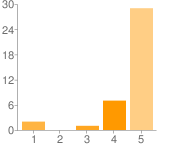
\includegraphics[scale=0.7]{images/encuesta2/8}
        \end{center}

	\item ¿Encuentra que TRAC cumple perfectamente
		su objetivo como herramienta central de
		gestión?

		\begin{verbatim}
        1		2		3		4		5
        No						Completamente de acuerdo
		\end{verbatim}
        \begin{center}
        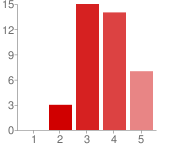
\includegraphics[scale=0.7]{images/encuesta2/9}
        \end{center}

	\item ¿Considera que la realización de proyectos
		internacionales es entorpecida por las
		distancias?
		\begin{verbatim}
         1		2		3		4		5
         No							Si, demasiado.
		\end{verbatim}
        \begin{center}
        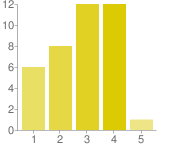
\includegraphics[scale=0.7]{images/encuesta2/10}
        \end{center}
	\item ¿Considera que TRAC permite una correcta
		administración de los recursos humanos?
		\begin{verbatim}
         1		2		3		4		5
         No, para nada.					Si.
		\end{verbatim}
        \begin{center}
        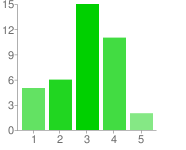
\includegraphics[scale=0.7]{images/encuesta2/11}
        \end{center}
	\item ¿Es Skype un buen mecanismo para la
		comunicación en reuniones? 
		\begin{verbatim}
         1	2	3	4	5
         No			Si, muy útil
		\end{verbatim}
        \begin{center}
        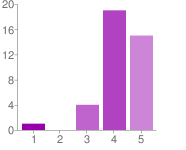
\includegraphics[scale=0.7]{images/encuesta2/12}
        \end{center}
	\item ¿Cuál de los siguientes softwares
		preferiría para la creación de documentos
		de forma distribuida:
		\begin{enumerate}
			\item LaTeX y Git/SVN
			\item Office (MS, OO)
			\item Google Docs
			\item Other: 
		\end{enumerate}
        \begin{center}
        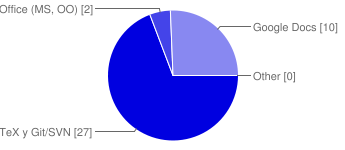
\includegraphics[scale=0.7]{images/encuesta2/13}
        \end{center}
	\item ¿Como discutiría usted la re-planificación
		de un proyecto determinado?
		\begin{enumerate}
			\item E-Mail
			\item Reunión presencial
			\item Reunión remota (teleconferencia)
			\item Other: 
		\end{enumerate}
        \begin{center}
        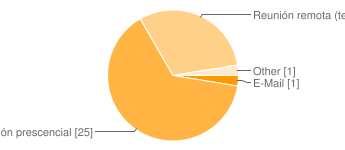
\includegraphics[scale=0.7]{images/encuesta2/14}
        \end{center}
	\item ¿Cual considera que es la mejor forma de
		motivar al equipo de trabajo?
		\begin{enumerate}
			\item Se felicita y premian los logros
			\item Se castiga el fracaso
			\item Se incentiva la creatividad y la generación de nuevos proyectos
			\item Incentivos monetarios al mejor trabajador del periodo
			\item Other: 
		\end{enumerate}
        \begin{center}
        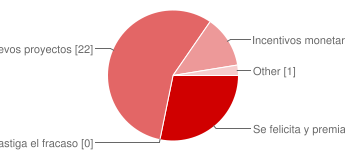
\includegraphics[scale=0.7]{images/encuesta2/15}
        \end{center}
\end{enumerate}

\subsubsection{Control y Monitoreo}

\begin{enumerate}
	\item ¿Que tan útil encuentra el uso de bitácoras
		diarias (worklogs)?

		\begin{verbatim}
         1	2	3	4	5
         Inútil		Muy Útil
		\end{verbatim}
        \begin{center}
        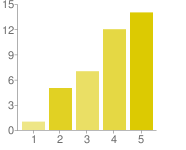
\includegraphics[scale=0.7]{images/encuesta2/16}
        \end{center}
	\item ¿Qué tan útil encuentra el realizar una reunión
		semanal por cada proyecto?

		\begin{verbatim}
        1	2	3	4	5
        Inútil	      Muy Útil
		\end{verbatim}
        \begin{center}
        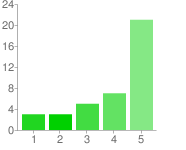
\includegraphics[scale=0.7]{images/encuesta2/17}
        \end{center}
	\item ¿Considera que las diferencias culturales son un
		impedimento para llevar un buen control?
		\begin{verbatim}
         1		2		3		4		5
         No, para nada				Si, mucho
		\end{verbatim}
        \begin{center}
        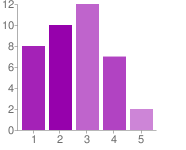
\includegraphics[scale=0.7]{images/encuesta2/18}
        \end{center}
	\item ¿Que tipo de control y monitoreo utiliza?
	\begin{enumerate}
 		\item Del tipo estático (programados cada 1 semana)
 		\item Del tipo dinámico (cuando sean necesarios)
 		\item Other: 
	\end{enumerate}
        \begin{center}
        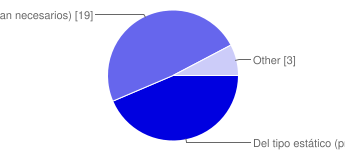
\includegraphics[scale=0.7]{images/encuesta2/19}
        \end{center}
\end{enumerate}

\subsubsection{Cierre}
\begin{enumerate}
	\item ¿Cree que un software (por ejemplo, trac) le
		permite un correcto seguimiento después de
		terminar un proyecto?
		\begin{verbatim}
        1	2	3	4	5
        No				Si
		\end{verbatim}
        \begin{center}
        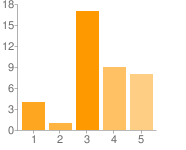
\includegraphics[scale=0.7]{images/encuesta2/20}
        \end{center}
	\item En proyectos internacionales, ¿Ha obtenido
		beneficios no relacionados con los proyectos
		(aprendizaje, culturales, oportunidades de
		trabajo) ?
		\begin{verbatim}
          1		2	3	4	5
          No			  Si, Mucho
		\end{verbatim}
        \begin{center}
        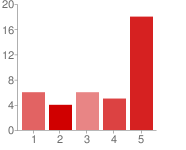
\includegraphics[scale=0.7]{images/encuesta2/21}
        \end{center}
	\item ¿Como se escogen las responsabilidades de cada
		persona encargada de la mantención de un proyecto?
		\begin{enumerate}
			\item Votación
			\item Desempeño
			\item Elección del jefe
			\item Other: 
		\end{enumerate}
        \begin{center}
        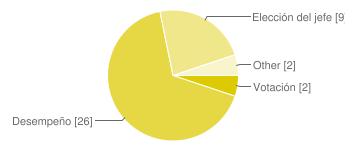
\includegraphics[scale=0.7]{images/encuesta2/22}
        \end{center}
\end{enumerate}

\subsection{Resultados Encuesta}

Entre una media de 40 encuestados, podemos concluir que:

\begin{enumerate}

\item \textbf{Inicio}\\
Con respecto al puntapié inicial de un proyecto, la gran mayoría reconoce al Brainstorming,
como la principal metodología para la generación de ideas. Por otro lado indican que
para la toma de decisiones se hace importante la participación de varios integrantes,
mediante una discusión abierta, rescatando lo bueno de cada propuesta. Por último se destaca
el hecho de que los Workshop de introducción son una de las metodologías mas utilizadas 
para la introducción de ciertos temas específicos a nuevos integrantes.

\item \textbf{Plan}\\
En lo que refiere al Plan, Se destaca que TRAC permite en forma eficiente, la correcta
planificación de un proyecto estándar. Complementando a ésto, señalan que un proyecto tiene
pocas posibilidades de alcanzar un éxito si no se realiza una planificación adecuada, salvo
en contados casos. Para la planificación temporal de cada actividad, indican que Planner es 
herramienta entre moderada y buena para dicha tarea.

\item \textbf{Ejecución}\\
Se puede apreciar como una buena y fluida comunicación es de vital importancia
para el éxito de un proyecto, por lo que se le da una gran importancia tanto a
las reuniones periódicas como a la discusión de las diferentes ideas que
puedan tener los miembros del equipo, evitando conflictos y resolviendo
problemáticas de forma dinámica. La distancia se puede considerar como un
punto importante que sí dificulta el desarrollo de un proyecto, pero cada vez
estas dificultades son menos, y las herramientas como Trac, sistemas de
control de versiones como Git y SVN, y Google Docs, ayudan a trabajar
colaborativamente sin importar la distancia físicas de las personas. Para la
planificación y discusión de ideas, que el equipo se reúna presencialmente o
digitalmente es de vital importancia, privilegiando las oportunidades de
reunión físicas por sobre las virtuales.

\item \textbf{Control y Monitoreo}\\
El realizar bitácoras y llevar registros de las actividades realizadas por
cada uno ayuda significativamente para el monitoreo y control del proyecto. El
confiar a la herramienta Trac por si sola es un error, siendo esta
insuficiente al momento de controlar y revisar las actividades realizadas
históricamente. Se vuelve a reiterar la importancia de las reuniones
periódicas, siendo las semanales las que darían un mejor resultado. Las
diferencias culturales no son un punto crítico al momento de llevar el control
del proyecto, indistintamente si se utilice un tipo de control estático o
dinámico, no existiendo una preferencia clara por uno de ellos. Por último,
la asignación de responsabilidades idealmente se asigna dependiendo de los méritos y el
desempeño de cada miembro, aunque la opinión y asignaciones realizadas por un
jefe del equipo siguen estando presentes en un 20\% de los casos. Cabe
destacar lo enriquecedoras que son las experiencias de trabajo en proyectos
internacionales, siendo estos no sólo dentro del área de la experticie, sino
también sociales y culturales.

\item \textbf{Cierre}\\
Por último, indican que un software para el seguimiento de un proyecto, permite un feedback moderado,
en lo que respecta a las actividades post-termino del proyecto. Un punto a destacar, es la obtención
de muchos beneficios no relacionados directamente con el proyecto, al momento de desarrollar
un proyecto internacional, refiriéndonos a beneficios culturales, oportunidades de trabajo, etc. 
No menos importante es el hecho de que se escogen las responsabilidades de cada persona encargada 
de la mantención de un proyecto, mediante la medición del desempeño.
\end{enumerate}
